\documentclass[11pt,oneside]{book}
\usepackage[T1]{fontenc}
%\usepackage[utf8]{inputenc}
\usepackage[a4paper]{geometry}
\usepackage[sectionbib]{natbib}
\usepackage{chapterbib}
\usepackage{graphicx}
\usepackage{hyperref}
%%% Uncomment if you change the bibliography heading/title
% \renewcommand{\bibname}{References}

%%% Uncomment if you want to include the bibliographies at the end of each chapter in the table of contents.  
% \usepackage[nottoc]{tocbibind}

\usepackage{xparse}

\usepackage[T1]{fontenc}
%\usepackage[utf8]{inputenc}
\usepackage[a4paper]{geometry}
%\usepackage[sectionbib]{natbib}
\usepackage{chapterbib}
\usepackage{graphicx}
\usepackage{hyperref}
\hypersetup{colorlinks=true, linkcolor=blue,  anchorcolor=blue,  
citecolor=blue, filecolor=blue, menucolor=blue,  
urlcolor=blue}
%%% Uncomment if you change the bibliography heading/title
% \renewcommand{\bibname}{References}

%%% Uncomment if you want to include the bibliographies at the end of each chapter in the table of contents.  
\usepackage[nottoc]{tocbibind}

\usepackage{xparse}

\let\oldsection\section
\makeatletter
\newcounter{@secnumdepth}
\RenewDocumentCommand{\section}{s o m}{%
  \IfBooleanTF{#1}
    {\setcounter{@secnumdepth}{\value{secnumdepth}}% Store secnumdepth
     \setcounter{secnumdepth}{0}% Print only up to \chapter numbers
     \oldsection{#3}% \section*
     \setcounter{secnumdepth}{\value{@secnumdepth}}}% Restore secnumdepth
    {\IfValueTF{#2}% \section
       {\oldsection[#2]{#3}}% \section[.]{..}
       {\oldsection{#3}}}% \section{..}
}
\makeatother

\makeatletter
\let\oldchapter\chapter
\RenewDocumentCommand{\chapter}{s o m}{%
  \IfBooleanTF{#1}
    {\setcounter{@secnumdepth}{\value{secnumdepth}}% Store secnumdepth
     \setcounter{secnumdepth}{0}% Print only up to \chapter numbers
     \oldchapter{#3}% \chapter*
     \setcounter{secnumdepth}{\value{@secnumdepth}}}% Restore secnumdepth
    {\IfValueTF{#2}% \chapter
       {\oldchapter[#2]{#3}}% \chapter[.]{..}
       {\oldchapter{#3}}}% \chapter{..}
}
\makeatother

%%%%%%%%%%%%%%%%%%%%%%%%%%%%%%%%%%%%%%%%%%%%%%%%%%%%%%%%%%%%%%%%%%%%%%%%%%%%%%%%
% 'dedication' environment: To add a dedication paragraph at the start of book %
% Source: http://www.tug.org/pipermail/texhax/2010-June/015184.html            %
%%%%%%%%%%%%%%%%%%%%%%%%%%%%%%%%%%%%%%%%%%%%%%%%%%%%%%%%%%%%%%%%%%%%%%%%%%%%%%%%
\newenvironment{dedication}
{
   \cleardoublepage
   \thispagestyle{empty}
   \vspace*{\stretch{1}}
   \hfill\begin{minipage}[t]{0.66\textwidth}
   \raggedright
}
{
   \end{minipage}
   \vspace*{\stretch{3}}
   \clearpage
}


%%%%%%%%%%%%%%%%%%%%%%%%%%%%%%%%%%%%%%%%%%%%%%%%
% Chapter quote at the start of chapter        %
% Source: http://tex.stackexchange.com/a/53380 %
%%%%%%%%%%%%%%%%%%%%%%%%%%%%%%%%%%%%%%%%%%%%%%%%
\makeatletter
\renewcommand{\@chapapp}{}% Not necessary...
\newenvironment{chapquote}[2][2em]
  {\setlength{\@tempdima}{#1}%
   \def\chapquote@author{#2}%
   \parshape 1 \@tempdima \dimexpr\textwidth-2\@tempdima\relax%
   \itshape}
  {\par\normalfont\hfill--\ \chapquote@author\hspace*{\@tempdima}\par\bigskip}
\makeatother



\usepackage[framemethod=TikZ]{mdframed}

% \newcounter{iframe}[chapter]\setcounter{iframe}{0}
% \renewcommand{\theiframe}{\arabic{chapter}.\arabic{iframe}}
\newenvironment{iframe}[1][]{%
% \refstepcounter{iframe}%
\ifstrempty{#1}%
{\mdfsetup{%
frametitle={%
\tikz[baseline=(current bounding box.east),outer sep=0pt]
\node[anchor=east,rectangle,fill=blue!20]
{\strut Digital Content};}}
}%
{\mdfsetup{%
frametitle={%
\tikz[baseline=(current bounding box.east),outer sep=0pt]
\node[anchor=east,rectangle,fill=blue!20]
{\strut Digital Content~:~#1};}}%
}%
\mdfsetup{innertopmargin=10pt,linecolor=blue!20,%
linewidth=2pt,topline=true,%
frametitleaboveskip=\dimexpr-\ht\strutbox\relax
}
\begin{mdframed}[]}{\end{mdframed}}



%%%%%%%%%%%%%%%%%%%%%%%%%%%%%%%%%%%%%%%%%%%%%%%%%%%%%%%%%%%%%%%%%%%%%%%%%%%%%%%%
% calchub environment: for embedding a calchub workspace                       %
% texedbook compatible: html=embedded work space, pdf=multimedia box w/ href   %
%%%%%%%%%%%%%%%%%%%%%%%%%%%%%%%%%%%%%%%%%%%%%%%%%%%%%%%%%%%%%%%%%%%%%%%%%%%%%%%%
\newenvironment{calchub}
    {\begin{iframe}[CalcHub Workspace]
    }
    {\end{iframe}
    }

\newcommand{\InsertCalchub}[3]{ 
   % 1st input: display name 
   % 2nd input: href
   % 3rd input: description
   \begin{calchub}
      \href{#2}{#1} | #3
   \end{calchub}
} 


%%%%%%%%%%%%%%%%%%%%%%%%%%%%%%%%%%%%%%%%%%%%%%%%%%%%%%%%%%%%%%%%%%%%%%%%%%%%%%%%
% video environment: for embedding videos                                      %
% texedbook compatible: html=embedded video, pdf=multimedia box w/ href        %
%%%%%%%%%%%%%%%%%%%%%%%%%%%%%%%%%%%%%%%%%%%%%%%%%%%%%%%%%%%%%%%%%%%%%%%%%%%%%%%%
\newenvironment{youtube}
   {\begin{iframe}[Video]
   }
   {\end{iframe}
   }

\newcommand{\InsertYoutube}[3]{ 
   % 1st input: display name 
   % 2nd input: href
   % 3rd input: description
   \begin{youtube}
      \href{#2}{#1} | #3
   \end{youtube}
} 

%%%%%%%%%%%%%%%%%%%%%%%%%%%%%%%%%%%%%%%%%%%%%%%%%%%%%%%%%%%%%%%%%%%%%%%%%%%%%%%%
% python coding environment: for coding practice                               %
% texedbook compatible: html=embedded trinket, pdf=multimedia box w/ href      %
%%%%%%%%%%%%%%%%%%%%%%%%%%%%%%%%%%%%%%%%%%%%%%%%%%%%%%%%%%%%%%%%%%%%%%%%%%%%%%%%


\newenvironment{trinket}
   {\begin{iframe}[Python coding environment]
   }
   {\end{iframe}
   }

\newcommand{\InsertTrinket}[3]{ 
   % 1st input: display name 
   % 2nd input: href
   % 3rd input: description
   \begin{trinket}
      \href{#2}{#1} | {#3}
   \end{trinket}
} 


%%%%%%%%%%%%%%%%%%%%%%%%%%%%%%%%%%%%%%%%%%%%%%%%%%%%%%%%%%%%%%%%%%%%%%%%%%%%%%%%
% panopto environment: for viewing videos hosted by panopto                    %
% texedbook compatible: html=embedded iframe, pdf=multimedia box w/ href       %
%%%%%%%%%%%%%%%%%%%%%%%%%%%%%%%%%%%%%%%%%%%%%%%%%%%%%%%%%%%%%%%%%%%%%%%%%%%%%%%%


\newenvironment{panopto}
   {\begin{iframe}[Video]
   }
   {\end{iframe}
   }

\newcommand{\InsertPanoptoVideo}[3]{ 
   % 1st input: display name 
   % 2nd input: href
   % 3rd input: description
   \begin{panopto}
      \href{#2}{#1} | {#3}
   \end{panopto}
} 





%%%%%%%%%%%%%%
% Title Page %
%%%%%%%%%%%%%%

% Book's title and subtitle
\title{\Huge \textbf{TexEdBook}}
% Authors
\author{\textsc{Riley Hanus}}

\begin{document}

\frontmatter
\maketitle

\chapter*{Forward}
This is \emph{not} a full thesis template! It only demonstrates how to create per-chapter references using the \texttt{chapterbib} package with BibTeX. (Do not use with BibLaTeX!)

Each chapter must be in its own \texttt{.tex} file and \texttt{include}-d into the main \texttt{.tex} file. If compiling on your own machine, run \texttt{bibtex} on \emph{each} generated \texttt{.aux} file, before running \texttt{pdflatex} twice more. (These are done automatically on Overleaf.)

\tableofcontents

\mainmatter

\chapter{Interactive Content}
Lorem ipsum dolor sit amet, consectetur adipisicing elit, sed do eiusmod tempor incididunt ut labore et dolore magna aliqua.

Ut enim ad minim veniam, quis nostrud exercitation ullamco laboris nisi ut aliquip ex ea commodo consequat.

\section{Videos}

% \InsertYoutubeVideo{Fourier Transforms}{https://www.youtube.com/watch?v=r6sGWTCMz2k}
\InsertYoutube{Calculus}{https://www.youtube.com/watch?v=WUvTyaaNkzM}

\section{Coding}

Duis aute irure dolor in reprehenderit in voluptate velit esse cillum dolore eu fugiat nulla pariatur. Excepteur sint occaecat cupidatat non proident, sunt in culpa qui officia deserunt mollit anim id est laborum. 


\begin{verbatim}
        import numpy as np
        import matplotlib.pyplot as plt

        x = np.linspace(0,2)
        y1 = np.exp(x)
        y2 = x + 1

        plt.plot(x, y1, label=r"$y_1=e^x$")
        plt.plot(x, y2, label=r"$y_2 = x + 1$")
        plt.legend()
        plt.xlim(0,1)
        plt.ylim(0,3)
        plt.xlabel('x')
        plt.ylabel('y')

        plt.show()
\end{verbatim}

\InsertTrinket{Sample Trinket}{https://trinket.io/embed/python3/e3a58e56a6}

\section{Live Math}

Duis aute irure dolor in reprehenderit in voluptate velit esse cillum dolore eu fugiat nulla pariatur. Excepteur sint occaecat cupidatat non proident, sunt in culpa qui officia deserunt mollit anim id est laborum. 


\InsertCalchub{Sample CalcHub Workspace}{https://calchub.co/calcs/16c5e5ef}
\bibliographystyle{unsrt}
\bibliography{sample}
\chapter{Equations and Figures }

\section{Equations}
Lorem ipsum dolor sit amet, $\kappa_\mathrm{pg}$
consectetur adipiscing elit. Duis risus ante, auctor et pulvinar non, posuere ac lacus. Praesent egestas nisi id metus rhoncus ac lobortis sem hendrerit Eq. \mjref{eq:Callaway}. Etiam et sapien eget lectus interdum posuere sit amet ac urna. Aliquam pellentesque imperdiet erat, eget consectetur felis malesuada quis. Pellentesque sollicitudin, odio sed dapibus eleifend, magna sem luctus turpis, id aliquam felis dolor eu diam. Etiam ullamcorper, nunc a accumsan adipiscing, turpis odio bibendum erat, id convallis magna eros nec metus. Sed vel ligula justo, sit amet vestibulum dolor. Sed vitae augue sit amet magna ullamcorper suscipit. Quisque dictum ipsum a sapien egestas facilisis.

\begin{equation}
  \kappa_\mathrm{pg}=\frac{1}{3} \intop _0 ^{\omega_\mathrm{max}} C(\omega) \, v_\mathrm{g}(\omega)^2 \, \tau(\omega) \, d\omega. \label{eq:Callaway}
\end{equation}

Test. Etiam ullamcorper, nunc a accumsan adipiscing, turpis odio bibendum erat, id convallis magna eros nec metus. Sed vel ligula justo, sit amet vestibulum dolor. Sed vitae augue sit amet magna ullamcorper suscipit. Quisque dictum ipsum a sapien egestas facilisis. 

\section{Figure}
\noindent Lorem ipsum dolor sit amet Figure \ref{fig:test}, consectetur adipiscing elit. Reference something in Chapter 1, Table \ref{table:nonlin}. Duis risus ante, auctor et pulvinar non, posuere ac lacus. Praesent egestas nisi id metus rhoncus ac lobortis sem hendrerit. Etiam et sapien eget lectus interdum posuere sit amet ac urna \citep{latex:companion}. Etiam et sapien eget lectus interdum posuere sit amet ac urna. Aliquam pellentesque imperdiet erat, eget consectetur felis malesuada quis. Pellentesque sollicitudin, odio sed dapibus eleifend, magna sem luctus turpis, id aliquam felis dolor eu diam. Etiam ullamcorper, nunc a accumsan adipiscing, turpis odio bibendum erat, id convallis magna eros nec metus. Sed vel ligula justo, sit amet vestibulum dolor. Sed vitae augue sit amet magna ullamcorper suscipit. Quisque dictum ipsum a sapien egestas facilisis. \href{http://thermoelectrics.matsci.northwestern.edu/}{Snyder's thermoelectrics website.}

\begin{figure}
  \centering
  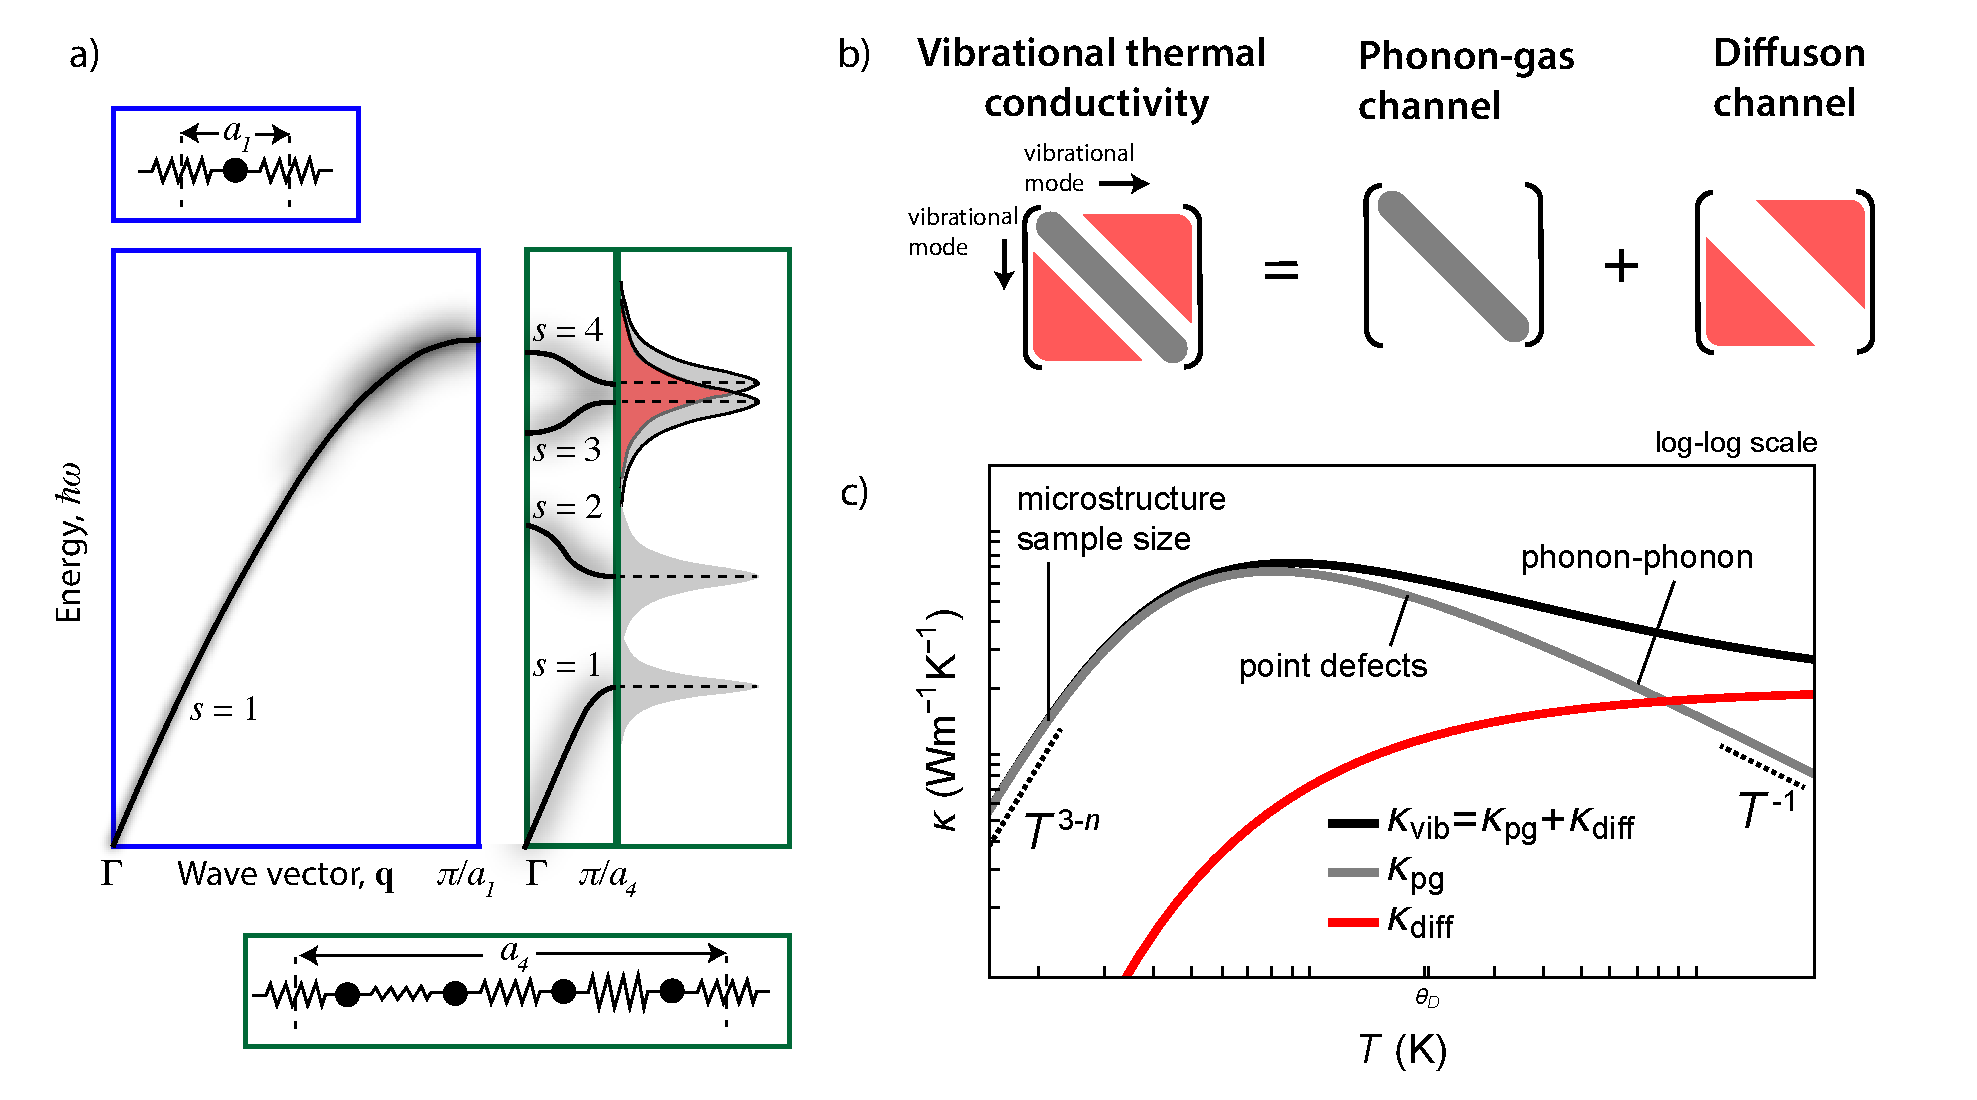
\includegraphics[width=0.99\textwidth, keepaspectratio]{figures/test-fig.pdf}
  \caption{Figure Lorem ipsum dolor sit amet, consectetur adipiscing elit. Duis risus ante, auctor et pulvinar non, posuere ac lacus. Praesent egestas nisi id metus rhoncus ac lobortis sem hendrerit.}
  \label{fig:test}
\end{figure}

%\bibliographystyle{unsrtnat}  %% For numerical citations remember to pass "numbers" option to natbib
\bibliographystyle{unsrt}
\bibliography{sample}


\chapter{Custom functions}
Lorem ipsum dolor sit amet, consectetur adipisicing elit, sed do eiusmod tempor incididunt ut labore et dolore magna aliqua.

Ut enim ad minim veniam, quis nostrud exercitation ullamco laboris nisi ut aliquip ex ea commodo consequat.

\section{YouTube}

% \InsertYoutubeVideo{Fourier Transforms}{https://www.youtube.com/watch?v=r6sGWTCMz2k}
\InsertYoutubeVideo{Calculus}{https://www.youtube.com/watch?v=WUvTyaaNkzM}

\section{CalcHub}

Duis aute irure dolor in reprehenderit in voluptate velit esse cillum dolore eu fugiat nulla pariatur. Excepteur sint occaecat cupidatat non proident, sunt in culpa qui officia deserunt mollit anim id est laborum. 

\InsertCalchubWorkspace{Sample CalcHub Workspace}{https://calchub.co/calcs/16c5e5ef}
\bibliographystyle{unsrt}
\bibliography{sample}


\backmatter
\chapter*{Afterword}
%\addcontentsline{toc}{chapter}{Additional Reading}
\nocite{lim:etal:kdtei:2016,markdown:overleaf}   % .bib keys of your own publications

{\renewcommand{\bibsection}{}
\bibliographystyle{dcu}
\bibliography{sample}
}


\end{document}
